%%%%%%%%%%%%%%%%%%%%%%% file template.tex %%%%%%%%%%%%%%%%%%%%%%%%%
%
% This is a general template file for the LaTeX package SVJour3
% for Springer journals.          Springer Heidelberg 2010/09/16
%
% Copy it to a new file with a new name and use it as the basis
% for your article. Delete % signs as needed.
%
% This template includes a few options for different layouts and
% content for various journals. Please consult a previous issue of
% your journal as needed.
%
%%%%%%%%%%%%%%%%%%%%%%%%%%%%%%%%%%%%%%%%%%%%%%%%%%%%%%%%%%%%%%%%%%%
%
% First comes an example EPS file -- just ignore it and
% proceed on the \documentclass line
% your LaTeX will extract the file if required
\begin{filecontents*}{example.eps}
%!PS-Adobe-3.0 EPSF-3.0
%%BoundingBox: 19 19 221 221
%%CreationDate: Mon Sep 29 1997
%%Creator: programmed by hand (JK)
%%EndComments
gsave
newpath
  20 20 moveto
  20 220 lineto
  220 220 lineto
  220 20 lineto
closepath
2 setlinewidth
gsave
  .4 setgray fill
grestore
stroke
grestore
\end{filecontents*}
%
\RequirePackage{fix-cm}
%
%\documentclass{svjour3}                     % onecolumn (standard format)
%\documentclass[smallcondensed]{svjour3}     % onecolumn (ditto)
\documentclass[smallextended]{svjour3}       % onecolumn (second format)
%\documentclass[twocolumn]{svjour3}          % twocolumn
%
\smartqed  % flush right qed marks, e.g. at end of proof
%
\usepackage{graphicx}
%
% \usepackage{mathptmx}      % use Times fonts if available on your TeX system
%
% insert here the call for the packages your document requires
%\usepackage{latexsym}
\usepackage{amsmath}
\usepackage{amssymb}

% etc.
%
% please place your own definitions here and don't use \def but
% \newcommand{}{}
%
% Insert the name of "your journal" with
% \journalname{myjournal}
%
\begin{document}

\title{Insert your title here%\thanks{Grants or other notes
%about the article that should go on the front page should be
%placed here. General acknowledgments should be placed at the end of the article.}
}
\subtitle{If you have a subtitle, write it here}

%\titlerunning{Short form of title}        % if too long for running head

\author{Shuai Fu         \and
        Nizar Bouguila %etc.
}

%\authorrunning{Short form of author list} % if too long for running head

\institute{Shuai Fu  \at
			  Concordia Institute for Information Systems Engineering					\\
              Concordia University, Montreal, Canada \\
              \email{f\_shuai@encs.concordia.ca}           %  \\
%             \emph{Present address:} of F. Author  %  if needed
           \and
           Nizar Bouguila \at
           	  Concordia Institute for Information Systems Engineering					\\
              Concordia University, Montreal, Canada \\
              \email{nizar.bouguila@concordia.ca}    
}

\date{Received: date / Accepted: date}
% The correct dates will be entered by the editor


\maketitle

\begin{abstract}
A novel unsupervised Bayesian learning framework based on asymmetric Gaussian mixture (AGM) statistical model is proposed since AGM is shown to be more effective compared to the classic Gaussian mixture. The Bayesian learning framework is developed by adopting sampling-based Markov chain Monte Carlo (MCMC) methodology. More precisely, the fundamental learning algorithm is a hybrid  Metropolis-Hastings within Gibbs sampling solution which is integrated within a reversible jump MCMC (RJMCMC) learning framework, a self-adapted sampling-based MCMC implementation, that enables model transfer throughout the mixture parameters learning process, therefore, automatically converges to the optimal number of data groups. Furthermore, considering the involvement of high-dimensional visual datasets, a dimensionality reduction algorithm based on mixtures of distributions is included to tackle the irrelevant and extraneous features. The performance comparison between AGM and other popular solutions is given and both synthetic and real data sets extracted from challenging applications such as intrusion detection, spam filtering and image categorization are evaluated to show the merits of the proposed approach.

\keywords{Asymmetric Gaussian Mixture \and RJMCMC \and Intrusion Detection \and Spam Filtering \and Image Categorization \and Dimensionality Reduction}
% \PACS{PACS code1 \and PACS code2 \and more}
% \subclass{MSC code1 \and MSC code2 \and more}
\end{abstract}

\section{Introduction}
\label{intro}
Over past decades, many statistical data mining approaches have been proposed to address challenging data modeling analysis problems given the fact that the volume of data is dramatically increasing due to the usage of Internet. Meanwhile, modern machine-learning-based techniques perform in both generative and discriminative ways which can be divided into two main streams, classification-based supervised and clustering-based unsupervised ones. Compared to supervised solutions, unsupervised approach has no assumption on the number of groups, therefore, friendly to newly added data and patterns which makes it more suitable for increasing database analysis. Moreover, it also immunizes against learning biases and overfitting problems that commonly exist in most supervised approaches if model training is inappropriate. Consequently, there has been an increasing trend of applying finite mixtures into different domains involving statistical modeling of data, such as astronomy, ecology, bioinformatics, pattern recognition, computer vision and machine learning \cite{Bouguila2006}. Our work is based on asymmetric Gaussian mixture (AGM) model \cite{Elguebaly2014} and reversible jump Markov chain Monte Carlo (RJMCMC) learning algorithm \cite{Richardson1997}. Previous efforts reveal the fact that AGM outperforms classic Gaussian mixture model (GMM) by taking asymmetric datasets into consideration which provides more flexibility \cite{Elguebaly2013}. Our RJMCMC implementation is based on a hybrid sampling-based approach which takes advantages of both Metropolis-Hastings (MH) and Gibbs sampling methods \cite{Elguebaly2011}, therefore, simplifies mathematical complexity and extends adaptability of the model. Moreover, without giving a fixed components number in advance, RJMCMC applies a dynamic data-based strategy to identify the optimal components number throughout iterations which makes the model learning a self-adaptive process. To achieve better fitting outcomes, feature selection process is involved to handle high-dimensional vectors of features and the analysis and discussion of deploying AGM to both synthetic datasets and real applications is given in the later chapters.

\subsection{Finite Mixture Models}
\label{sec:1.1}
As upgrade of single-mathematical-model-based methodologies, mixture models \cite{Yang2015,Wen2015,Bouguila2011a} can be seen as a superimposition of certain mixture components sharing dependencies with each other, therefore, lead to outstanding performance especially for high-dimensional and multi-cluster datasets. Finite mixture models can be described by
\begin{equation}
p(X|\Theta) = \sum_{j=1}^Mp_jp(X|\Theta_j)
\label{eq:finiteMixture}
\end{equation}

where $X$ reprensents a vector in a given dataset and $\Theta$ defines the mixture parameters set (for each mixture compoent, the sub-parameter set is described by $\Theta_j, j=1,\dots,M$) as well as component weight $p_j$ (0 $< p_j \leq$ 1 and $\sum_{j=1}^Mp_j$ = 1).

\subsection{Finite Mixture Models}
\label{sec:1.2}
Probability density function (PDF) selection has an important role in finite mixture model because it significantly affects the capability of representing the data. Improper PDF selection will cause incorrect outcomes such as wrong components number and poor data fitting. Gaussian mixture model (GMM) \cite{Richardson1997} demonstrated satisfactory fitting abilities on most real applications whose datasets are Gaussian-like. However, under more general circumstances regarding to non-Gaussian or asymmetric datasets, asymmetric Gaussian mixture (AGM) model \cite{Elguebaly2014} leads to a better accuracy by introducing two variance parameters for both left and right parts of asymmetric Gaussian distribution, providing more flexibility for variant real applications. Therefore, the justification of choosing AGM model and its merits will be discussed in the following chapters.

\subsection{Bayesian Learning Framework}
\label{sec:1.3}
Estimating the parameters of mixture models could be a challenging task. The maximum-likelihood-based expectation maximization (EM) \cite{Dempster1977} algorithm is one of the most popular parameter learning approaches. However, the disadvantages of EM algorithm are also obvious. Given the fact that EM approximates values of mixture parameters in a deterministic way this could cause slow convergence and compromise the usability of the algorithm. Furthermore, bad initialization and overfitting problems \cite{Bouguila2009,Bouguila2012} will also significantly affect its accuracy. Therefore, fully Bayesian learning algorithms, such as Markov Chain Monte Carlo (MCMC) based implementations, are found to be useful to eliminate overfitting problems in mixture parameter learning by introducing prior and posterior distributions for mixture parameters. In our work, the learning process is accomplished by a hybrid MCMC algorithm, which is well known as Metropolis-Hastings within Gibbs sampling \cite{Bouguila2009,Bourouis2014}, based on both Metropolis-Hastings \cite{Hastings1970} and Gibbs sampling \cite{Geman1987} methods because the main difficulty of classic MCMC method is that, under some circumstances, direct sampling is not always straightforward. Moreover, we reinforce the learning algorithm by introducing reversible jump MCMC (RJMCMC) \cite{Richardson1997} methodology to increase the flexibility of AGM model by allowing model transfer throughout iterations via increasing (component birth/split step) and decreasing (component death/merge step) mixture components. Because of the stochastic sampling-based learning process, learning iterations could end up with different number of components so we choose marginal likelihood \cite{Bouguila2009} to perform model selection in order to evaluate fitting results between models.

\subsection{Dimensionality Reduction}
\label{sec:1.4}

One of the most important tasks in data mining, pattern recognition, computer vision and machine learning applications is that, the existence of outliers and irrelevant features severely compromises the clustering outcomes. Therefore, many dimensionality reduction methodologies have been proposed \cite{Bouguila2011b,Boutemedjet2009} such as feature extraction and selection which try to remove these unneeded features in order to improve the performance of the modeling \cite{Raudys1991,Kohavi1997} while feature extraction is based on transformations or combinations of the original features \cite{Mao2005}. Indeed, feature selection methods identify relevant features in the original representation space. Recently, a volume of literature \cite{Tsai2008,Dy2004} has shown that selecting relevant features leads to more accurate modeling results. However, this problem is not trivial especially in the unsupervised context dealing with labelless data sets. For this reason, previous researches \cite{Law2004,Elguebaly2013,Elguebaly2015} were devoted to extend unsupervised feature selection to mixture-based clustering. In this article, we extended the RJMCMC-based simultaneous Bayesian clustering and feature selection approach proposed in \cite{Elguebaly2013} to asymmetric Gaussian mixture model in order to improve the modeling performance on a challenging image categorization application.

\subsection{Overview}
\label{sec:1.5}
The rest of this article is organized as follows:

\paragraph{Chapter 2} introduces the Asymmetric Gaussian mixture model and its sampling based Bayesian learning framework. In particular, a self-adapted reversible jump MCMC implementation which has no assumption concerning the number of components and, therefore, the AGM model itself could be transferred between iterations. Furthermore the self-adapted learning process treats components number as an extra parameter and adjusts it throughout iterations by automatically increasing (component birth/death step) and decreasing (component merge/split step) according to current status, therefore, enables model transfer which significantly improves the learning performance.
\paragraph{Chapter 3} is devoted to feature selection since the AGM model assumes that all the features of observations have the same weight of importance and carry pertinent information which is not always the case and many of those features can be irrelevant for clustering purpose. In order to tackle this problem and define relevance and importance of features, feature selection techniques should be taken into consideration. A challenging UIUC sports event database is selected for validation of the proposed approach.
\paragraph{Chapter 4} concludes and summarizes the article and points out future research directions.

\section{Asymmetric Gaussian Mixtures with Reversible Jump MCMC and Applications}
\label{sec:2}
This chapter presents a novel intrusion detection classifier based on asymmetric Gaussian mixture (AGM) model and reversible jump Markov chain Monte Carlo (RJMCMC) learning algorithm. Previous efforts reveal the fact that AGM outperforms classic Gaussian mixture model (GMM) by taking asymmetric datasets into consideration which provides more flexibility. Our RJMCMC implementation is based on a hybrid sampling-based approach which takes advantages of both Metropolis-Hastings (MH) and Gibbs sampling methods, therefore, simplifies mathematical complexity and extends adaptability of the model. Moreover, without giving a fixed components number in advance, RJMCMC applies a dynamic data-based strategy to identify the optimal components number throughout iterations which makes the model learning a self-adaptive process. Since the model is nondeterministic, Laplace approximation based marginal likelihood is calculated for multiple runs as model selection procedure to improve the correctness and fitting accuracy. Both synthetic and real datasets are applied to our model to discover its merits and the test results will be evaluated and compared with other popular solutions.

\subsection{Asymmetric Gaussian Mixture Model}
\label{sec:2.1}
The likelihood function of AGM model \cite{Elguebaly2014} with $M$ mixture components can be illustrated as follows:

\begin{equation}
p(\mathcal{X}|\Theta) = \prod_{i=1}^N \sum_{j=1}^Mp_jp(X_i|\xi_j)
\label{eq:likelihood}
\end{equation}

where $\mathcal{X} = (X_1,...,X_N)$ reprensents the dataset with $N$ observations, $\Theta = \{p_1,...,p_M, \xi_1,...,\xi_M\}$ defines the mixture parameters set of AGM mixture model including component weight $p_j$ (0 $< p_j \leq$ 1 and $\sum_{j=1}^Mp_j$ = 1) and asymmetric Gaussian distribution (AGD) parameters set $\xi_j$ for mixture component $j$. Assuming the dataset $\mathcal{X}$ is $d$-dimensional, for each observation $X_n = (x_{n1},...,x_{nd})\in\mathcal{X}$, the probability density function \cite{Elguebaly2014} for $j$-th component of the model can be defined as follows:

\begin{equation}
p(X|\xi_j) \propto \prod_{k=1}^{d} \frac{1}{(\sigma_{l_{jk}}+\sigma_{r_{jk}})}
\times \left\{\begin{matrix}
\exp \begin{bmatrix}
-\frac{(x_k-\mu_{jk})^2}{2(\sigma_{l_{jk}})^2}
\end{bmatrix}\ if\ x_k\ <\ \mu_{jk} \\ 
\exp \begin{bmatrix}
-\frac{(x_k-\mu_{jk})^2}{2(\sigma_{r_{jk}})^2}
\end{bmatrix}\ if\ x_k\ \geqslant\ \mu_{jk} \\ 
\end{matrix}\right.
\label{eq:2}
\end{equation}

parameters set of component $j$ is $\xi_j = (\mu_j,\sigma_{lj},\sigma_{rj})$ where $\mu_j = (\mu_{j1},...,\mu_{jd})$ is the mean, $\sigma_{lj} = (\sigma_{lj1},...,\sigma_{ljd})$ and $\sigma_{rj} = (\sigma_{rj1},...,\sigma_{rjd})$ represents the left and right standard deviation vectors of AGD . 

We bring a $M$-dimensional membership vector $Z$ to each observation $X_i\in\mathcal{X}, Z_i = (Z_{i1},...,Z_{iM})$, indicating which specific component $X_i$ belongs to \cite{Bouguila2006}, such that:
\begin{equation}
Z_{ij} = \left\{\begin{matrix}
1\qquad\mbox{ if }X_i\mbox{  belongs to component }j \\
0\qquad\qquad\quad \mbox{otherwise} \qquad\qquad\quad\quad \\
\end{matrix}\right.
\label{eq:memVector}
\end{equation}
that being said, $Z_{ij} = 1$ only when observation $X_i$ has the highest probability of belonging to component $j$ and accordingly, for other components, $Z_{ij} = 0$. 

Hence, the complete likelihood function can be obtained by combining Eq. \eqref{eq:likelihood} and Eq. \eqref{eq:memVector} as follows:
\begin{equation}
p(\mathcal{X}, Z|\Theta) = \prod_{i=1}^{N}\prod_{j=1}^{M}(p_jp(X_i|\xi_j))^{Z_{ij}}
\label{eq:compPdf}
\end{equation}

\subsection{Bayesian Learning Algorithm}
\label{sec:2.2}
Before describing MH-within-Gibbs learning steps, the priors and posteriors need to be specified. First, we denote the postorior probability of membership vector Z as $\pi(Z|\Theta,\mathcal{X})$ \cite{Elguebaly2011}:
\begin{equation}
Z \sim \pi(Z|\Theta^{(t-1)},\mathcal{X})
\label{eq:5}
\end{equation}
the number of observations belonging to a specific component $j$ can be calculated using $Z$ as follows:
\begin{equation}
n_j^{(t-1)} = \sum_{i=1}^NZ_{ij}\ (j = 1,...,M) 
\label{eq:6}
\end{equation}
thus $n^{(t-1)}=(n_1^{(t-1)},...,n_M^{(t-1)})$ represents the number of observations belonging to each mixture component.

Since the mixture weight $p_j$ satisfies the following conditions (0 $< p_j \leq$ 1 and $\sum_{j=1}^Mp_j$ = 1), a natural choice of the prior is Dirichlet distribution as follows \cite{Bouguila2004,Bouguila2004a} 
\begin{equation}
\pi(p_1,\ldots,p_M) \sim \mathcal{D}(\gamma_1,...,\gamma_M )
\label{eq:7}
\end{equation}
where $\gamma_j$ is known hyperparameter. Consequently, the posterior of the mixture weight $p_j$ is:
\begin{equation}
p(p_1,\ldots,p_M|Z) \sim \mathcal{D}(\gamma_1 + n_1^{(t-1)},...,\gamma_M + n_M^{(t-1)})
\label{eq:8}
\end{equation}


Direct sampling of mixture parameters $\xi \sim p(\xi|Z,\mathcal{X})$ could be difficult so Metropolis-Hastings method should be deployed using proposal distributions for $\xi^{(t)} \sim q(\xi|\xi^{(t-1)})$. To be more specific, for parameters of AGM model which are $\mu$ , $\sigma_l$ and $\sigma_r$, we choose proposal distributions as follows:
\begin{equation}
\mu_j^{(t)} \sim \mathcal{N}_d(\mu_j^{(t-1)},\Sigma)
\label{eq:9}
\end{equation}
\begin{equation}
\sigma_{lj}^{(t)} \sim \mathcal{N}_d(\sigma_{lj}^{(t-1)},\Sigma)
\label{eq:10}
\end{equation}
\begin{equation}
\sigma_{rj}^{(t)} \sim \mathcal{N}_d(\sigma_{rj}^{(t-1)},\Sigma)
\label{eq:11}
\end{equation}
the proposal distributions are $d$-dimensional Gaussian distributions with $\Sigma$ as $d$ x $d$ identity matrix which makes the sampling a random walk MCMC process.

As the most important part of Metropolis-Hastings method, at the end of each iteration, for new generated mixture parameter set $\Theta^{(t)}$, an acceptance ratio $r$ needs to be calculated in order to make a decision whether they should be accepted or discarded for the next iteration. The acceptance ratio $r$ is given by:
\begin{equation}
r = \frac{p(\mathcal{X}|\Theta^{(t)})\pi(\Theta^{(t)})q(\Theta^{(t-1)}|\Theta^{(t)})}{p(\mathcal{X}|\Theta^{(t-1)})\pi(\Theta^{(t-1)})q(\Theta^{(t)}|\Theta^{(t-1)})}
\label{eq:12}
\end{equation}

where $\pi(\Theta)$ is the proposed prior distribution which can be decomposed to $d$-dimensional Gaussian distributions such that $\mu \sim \mathcal{N}_d(\eta,\Sigma)$ and $\sigma_l, \sigma_r \sim \mathcal{N}_d(\tau,\Sigma)$ given known hyperparameters $\eta$ and $\tau$. The derivation of acceptance ratio $r$ is based on the assumption that mixture parameters are independent from each other which means that:

\bigskip
\begin{multline}
\pi(\Theta) = \pi(p,\xi) = \pi(\xi) = \prod_{j=1}^M\pi(\mu_j)\pi(\sigma_{lj})\pi(\sigma_{rj})\\
= \prod_{j=1}^M\mathcal{N}_d(\mu_j|\eta,\Sigma)\mathcal{N}_d(\sigma_{lj}|\tau,\Sigma)\mathcal{N}_d(\sigma_{rj}|\tau,\Sigma)\quad
\label{eq:14}
\end{multline}
in Eq. \eqref{eq:14}, since the mixture weigh $p$ is generated following Gibbs sampling method whose acceptance ratio is always 1, it should be excluded from Metropolis-Hastings estimation step. Accordingly, apply the same rule to the proposal distribution as well:
\begin{multline}
q(\Theta^{(t)}|\Theta^{(t-1)}) = q(\xi^{(t)}|\xi^{(t-1)}) \\
= \prod_{j=1}^M\mathcal{N}_d(\mu_j^{(t)}|\mu_j^{(t-1)},\Sigma)\mathcal{N}_d(\sigma_{lj}^{(t)}|\sigma_{lj}^{(t-1)},\Sigma)\mathcal{N}_d(\sigma_{rj}^{(t)}|\sigma_{rj}^{(t-1)},\Sigma)
\label{eq:15}
\end{multline}
by combining Eqs. \eqref{eq:2} \eqref{eq:compPdf} \eqref{eq:9} \eqref{eq:10} \eqref{eq:11} \eqref{eq:14} and \eqref{eq:15}, equation \eqref{eq:12} can be written as follows:

\begin{multline}
r = \frac{p(\mathcal{X}|\Theta^{(t)})\pi(\Theta^{(t)})q(\Theta^{(t-1)}|\Theta^{(t)})}{p(\mathcal{X}|\Theta^{(t-1)})\pi(\Theta^{(t-1)})q(\Theta^{(t)}|\Theta^{(t-1)})} = \prod_{i=i}^N \prod_{j=1}^M(\frac{p(X_i|\mu_j^{(t)},\sigma_{lj}^{(t)},\sigma_{rj}^{(t)})}
{p(X_i|\mu_j^{(t-1)},\sigma_{lj}^{(t-1)},\sigma_{rj}^{(t-1)})} \\
\times \frac{\mathcal{N}_d(\mu_j^{(t)}|\eta,\Sigma)\mathcal{N}_d(\sigma_{lj}^{(t)}|\tau,\Sigma)\mathcal{N}_d(\sigma_{rj}^{(t)}|\tau,\Sigma)}{\mathcal{N}_d(\mu_j^{(t-1)}|\eta,\Sigma)\mathcal{N}_d(\sigma_{lj}^{(t-1)}|\tau,\Sigma)\mathcal{N}_d(\sigma_{rj}^{(t-1)}|\tau,\Sigma)} \\
\times \frac{\mathcal{N}_d(\mu_j^{(t-1)}|\mu_j^{(t)},\Sigma)\mathcal{N}_d(\sigma_{lj}^{(t-1)}|\sigma_{lj}^{(t)},\Sigma)\mathcal{N}_d(\sigma_{rj}^{(t-1)}|\sigma_{rj}^{(t)},\Sigma)}{\mathcal{N}_d(\mu_j^{(t)}|\mu_j^{(t-1)},\Sigma)\mathcal{N}_d(\sigma_{lj}^{(t)}|\sigma_{lj}^{(t-1)},\Sigma)\mathcal{N}_d(\sigma_{rj}^{(t)}|\sigma_{rj}^{(t-1)},\Sigma)})
\label{eq:16}
\end{multline}
    
Once acceptance ratio $r$ is derived by Eq. \eqref{eq:16}, we compute acceptance probability $\alpha = min[1,r]$ \cite{Luengo2013}. Then $u \sim U_{[0,1]}$ is supposed to be generated randomly. If $\alpha < u$, the proposed move should be accepted and parameters should be updated by $p^{(t)}$ and $\xi^{(t)}$ for next iteration. Otherwise, we discard $p^{(t)}$, $\xi^{(t)}$ and set $p^{(t)} = p^{(t-1)}$, $\xi^{(t)} = \xi^{(t-1)}$.

We summarize the MH-within-Gibbs learning process for AGM model in the following steps:
\bigbreak
\noindent\textbf{Input:} Data observations $\mathcal{X}$ and components number $M$ \\
\textbf{Output:} AGM mixture parameter set $\Theta$
\bigbreak

\begin{enumerate}
\item Initialization
\item Step $t$: For $t = 1,\ldots$
\begin{enumerate}
\item[]\textbf{Gibbs sampling part}
\item Generate $Z^{(t)}$ from Eq. \eqref{eq:5}
\item Compute $n_j^{(t)}$ from Eq. \eqref{eq:6}
\item Generate $p_j^{(t)}$ from Eq. \eqref{eq:8}
\item[] \textbf{Metropolis-Hastings part}
\item Sample $\xi_j^{(t)}$ ($\mu_j^{(t)}, \sigma_{lj}^{(t)}, \sigma_{rj}^{(t)}$) from Eqs. \eqref{eq:9} \eqref{eq:10} \eqref{eq:11}
\item Compute acceptance ratio $r$ from Eq. \eqref{eq:12}
\item Generate $\alpha = min[1,r]$ and $u \sim U_{[0,1]}$
\item If $u \geq \alpha$ then $\xi^{(t)} = \xi^{(t-1)}$
\end{enumerate}
\end{enumerate}
\bigskip

\subsection{Reversible Jump Markov Chain Monte Carlo}
\label{sec:2.3}

We reinforce the learning algorithm by introducing reversible jump MCMC (RJMCMC) \cite{Bouguila2012} methodology to increase the flexibility of AGM model because traditional MH-within-Gibbs algorithm assumes that the component number $M$ is given and persistent throughout the learning process. However, because of bad initialization or just information leakage, $M$ could be inaccurate or unknown. Under these circumstances, RJMCMC algorithm presents its merits by providing extra four independent steps (birth/death steps and merge/split steps) into learning process which could change component number $M$, therefore, brings more generalities. 

In practice, within every RJMCMC learning iteration, the current component number $m$ is considered as an extra parameter which has a proposed Poisson prior $\mathcal{P}(\lambda)$ with $\lambda = 4$ particularly in our case \cite{Richardson1997}. Accordingly, let $M_{min}$ and $M_{max}$ denote the minimum and maximum number of components $M$, and assume the probabilities of performing birth/split and death/merge steps are $b_m$ and $d_m = 1 - b_m$ for $m = M_{min},\dots,M_{max}$ respectively. Obviously, $b_{M_{max}}=0$ and $d_{M_{min}}=0$. Correspondingly, $d_{M_{max}}=1-b_{M_{max}} = 1$ and $b_{M_{min}}=1-d_{M_{min}}=1$. For $m=M_{min}+1,\dots,M_{max}-1$, for simplification purpose, we choose the same value for both $b_m$ and $d_m$ as $b_m=d_m=0.5$. Within every iteration, we generate a random value $u' \sim U_{[0,1]}$ respectively for the four RJMCMC steps. If $b_m >= u'$ or $d_m >= u'$, birth/split or death/merge steps should be performed correspondingly \cite{Richardson1997}.

\textbf{Merge and Split Steps}: Randomly choose two components $(j_1,j_2)$ satisfying that $\mu_{j_1}<\mu_{j_2}$ with no other $\mu_j$ in the interval $[\mu_{j_1},\mu_{j_2}]$. The newly merged component $j'$ will contain the observations that previously belonged to both component $j_1$ and $j_2$. Meanwhile, reduce current value of component number $m$ to $m-1$, then calculate mixture weight and parameters for $j'$ as follows:
\begin{multline}
\qquad\qquad\qquad\qquad\qquad p_{j'} = p_{j_1}+p_{j_2} \\
p_{j'}\mu_{j'} = p_{j_1}\mu_{j_1} + p_{j_2}\mu_{j_2} \qquad\quad\\
p_{j'}(\mu_{j'}^2 + \sigma_{j'l}^2) = p_{j_1}(\mu_{j_1}^2 + \sigma_{j_1l}^2) + p_{j_1}(\mu_{j_1}^2 + \sigma_{j_1l}^2) \\
p_{j'}(\mu_{j'}^2 + \sigma_{j'r}^2) = p_{j_1}(\mu_{j_1}^2 + \sigma_{j_1r}^2)+p_{j_1}(\mu_{j_1}^2 + \sigma_{j_1r}^2)\qquad\quad
\label{eq:merge}
\end{multline}

As a reverse of merge step, we split component $j'$ into two ($j_1$ and $j_2$) with 3 degrees of freedom $(u_1 \sim Beta(2,2), u_2 \sim Beta(2,2), u_3 \sim Beta(1,1))$ and, accordingly, increase $m$ to $m+1$. Therefore, mixture parameters for split components can be calculated as follows:
\begin{multline}
\qquad\qquad\qquad\qquad\qquad p_{j_1} = p_{j'}u_1, p_{j_2} = p_{j'}u_2 \\
\mu_{j_1} = \mu_{j'} - \frac{u_2(\sigma_{j'l}+\sigma_{j'r})}{2} \sqrt{\frac{p_{j_2}}{p_{j_1}}} \\
\mu_{j_2} = \mu_{j'} + \frac{u_2(\sigma_{j'l}+\sigma_{j'r})}{2} \sqrt{\frac{p_{j_1}}{p_{j_2}}} \\
\sigma_{j_1l}^2 = u_3(1-u_2^2)\sigma_{j'l}^2\frac{p_{j'}}{p_{j_1}} \\
\sigma_{j_1r}^2 = u_3(1-u_2^2)\sigma_{j'r}^2\frac{p_{j'}}{p_{j_1}} \\
\sigma_{j_2l}^2 = (1-u_3)(1-u_2^2)\sigma_{j'l}^2\frac{p_{j'}}{p_{j_2}} \\
\sigma_{j_2r}^2 = (1-u_3)(1-u_2^2)\sigma_{j'r}^2\frac{p_{j'}}{p_{j_2}} \qquad\qquad\qquad\qquad
\label{eq:split}
\end{multline}

In order to decide whether the merge and split steps should be accepted or not, the acceptance probability \cite{Richardson1997} can be derived as follows: 

\begin{multline}
\qquad\qquad \mathcal{A}=\frac{p(\mathcal{X},Z|\Theta')}{p(\mathcal{X},Z|\Theta)}\frac{m'\mathcal{P}(m'|\lambda)}{\mathcal{P}(m|\lambda)}\frac{p_{j_1}^{\gamma-1+n_1}p_{j_2}^{\gamma-1+n_2}}{p_{j'}^{\gamma-1+n_1+n_2}Beta(\gamma,m\gamma)} \\
\times \sqrt{\frac{\kappa}{2\pi}} \exp[-\frac{1}{2}\kappa{(\mu_{j_1}-\xi)+(\mu_{j_2}-\xi)+(\mu_{j'}-\xi)}] \\
\times \frac{\beta^{\alpha}}{\Gamma(\alpha)}(\frac{\sigma_{j_1l}^2\sigma_{j_1r}^2\sigma_{j_2l}^2\sigma_{j_2r}^2}{\sigma_{j'l}^2\sigma_{j'r}^2})^{-\alpha-1} \qquad\qquad\qquad\qquad\\
\times \exp [{-\beta(\sigma_{j_1l}^2+\sigma_{j_1r}^2+\sigma_{j_2l}^2+\sigma_{j_2r}^2-\sigma_{j'l}^2-\sigma_{j'r}^2)}] \\
\qquad\times \frac{d_{m'}}{b_mP_{alloc}} [Beta(\mu_1|2,2)Beta(\mu_2|2,2)Beta(\mu_3|1,1)]^{-1} \\
\times \frac{p_{j'}|\mu_{j_1}-\mu_{j_2}|\sigma_{j_1l}^2\sigma_{j_1r}^2\sigma_{j_2l}^2\sigma_{j_2r}^2}{\mu_2(1-\mu_2^2)\mu_3(1-\mu_3)\sigma_{j'l}^2\sigma_{j'r}^2} \qquad\qquad\qquad\qquad\qquad\quad
\label{eq:acptProMS}
\end{multline}
where $\Theta'$ and $m' = m + 1$ denote the mixture parameters set and the component number respectively before merge or after split steps. $\kappa$ is a known hyperparameter and $\xi$ is the midpoint of the variation interval of the involved data observations. Besides, $P_{alloc}$ is the probability of which this particular allocation is made. Therefore, the acceptance probability for merge step is $\min(1,\mathcal{A})$ and, correspondingly, for split step is $\min(1,\mathcal{A}^{-1})$.

\textbf{Birth and Death Steps}: Compared to merge and split steps, birth and death steps are relatively straightforward because the newborn and dead components are empty ones which means parameter re-calculation is not needed. Mixture weight $p_{new}$ in birth step can be obtained by sampling from Beta distribution $p_{new} \sim Beta(1,m)$ and mixture parameters can be derived from the priors as follows \cite{Casella2004}:
\begin{align}
\mu \sim \mathcal{N}(\xi,\kappa^{-1}), \quad \sigma_{l}^{-2},\sigma_{r}^{-2} \sim \Gamma(\alpha,\beta), \quad \beta \sim \Gamma(g,h)
\label{eq:prior}
\end{align}
where hyperparameters $\kappa$, $\alpha$, $g$ and $h$ are chosen according to the data. For death step, an empty component should be randomly selected and deleted among the existing components if there is any. Otherwise, this step will be skipped. After birth and death steps, mixture weights $p_j$ should be re-scaled so that all weights sum to 1. Acceptance probability for birth and death steps is also required as the one for merge and split steps whose definition is as follows:

\begin{multline}
\mathcal{A}'=\frac{\mathcal{P}(m'|\lambda)}{\mathcal{P}(m|\lambda)}\frac{1}{Beta(m\gamma,\gamma)}p_{j'}^{\gamma-1}(1-p_{j'})^{N+m\gamma-m} \\
\times m' \frac{d_{m'}}{(m_0+1)b_m}\frac{1}{Beta(p_{j'}|1,m)}(1-p_{j'})^m
\label{eq:acptProBD}
\end{multline}
where $m_0$ is the amount of empty components. Thus, the probabilities of occurrence of birth and death steps are $\min(1,\mathcal{A}')$ and $\min(1,\mathcal{A}'^{-1})$ \cite{Richardson1997}.

Finally, Figure \ref{fig:DAG_rjmcmc} describes the dependencies between constants and variables involved in the Bayesian network of RJMCMC mixture parameter learning, and then, a typical learning procedure of AGM can be summarized as follows:

\begin{figure}
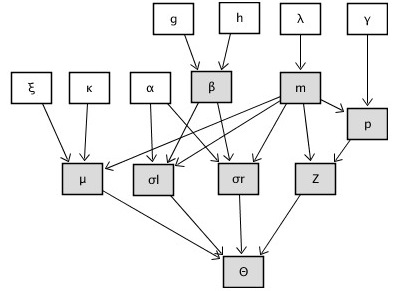
\includegraphics[width=0.75\textwidth]{DAG_RJMCMC.jpg}
\caption{DAG of RJMCMC parameter learning Bayesian network}
\label{fig:DAG_rjmcmc}
\end{figure}

\noindent\textbf{Input:} Data observations $\mathcal{X}$ and component number $M$ \\
\textbf{Output:} AGM mixture parameter set $\Theta$
\begin{enumerate}
\item Initialization
\item Step $t$: For $t = 1,\ldots$
\begin{enumerate}
\item[]\textbf{Gibbs sampling part}
\item Generate $Z^{(t)}$ from Eq. \eqref{eq:memVector}
\item Compute $n_j^{(t)}$ from Eq. \eqref{eq:6}
\item Generate $p_j^{(t)}$ from Eq. \eqref{eq:8}
\item[] \textbf{Metropolis-Hastings part}
\item Sample $\xi_j^{(t)}$ ($\mu_j^{(t)}, \sigma_{lj}^{(t)}, \sigma_{rj}^{(t)}$) from Eqs. \eqref{eq:9} \eqref{eq:10} \eqref{eq:11}
\item Compute acceptance ratio $r$ from Eq. \eqref{eq:12}
\item Generate $\alpha = min[1,r]$ and $u \sim U_{[0,1]}$
\item If $u \geq \alpha$ then $\xi^{(t)} = \xi^{(t-1)}$
\item[] \textbf{RJMCMC part}
\item Generate $u' \sim U_{[0,1]}$. If $b_m>=u'$, perform split or birth step, then calculate acceptance probability $\mathcal{A}$. If the step is accepted, set $m=m+1$.
\item Generate $u' \sim U_{[0,1]}$. If $d_m>=u'$, perform merge or death step, then calculate acceptance probability $\mathcal{A}'$. If the step is accepted, set $m=m-1$.
\end{enumerate}
\end{enumerate}

\subsection{Model Selection}
\label{sec:2.4}
Theoretically, RJMCMC learning process should always be able to derive the optimal components number $M$. However, because of the stochastic sampling, improper proposal distributions or bad initialization parameters, learning result based on a single estimation run is not always satisfactory. In order to establish a robust parameter estimation algorithm, we evaluate the estimation outputs derived from multiple RJMCMC runs with different initial values of components number by calculating their marginal likelihood with the Laplace approximation \cite{Bouguila2009} on the logarithm scale which is defined as follows:

\begin{multline}
\log(p(\mathcal{X}|M)) = \log(p(\mathcal{X}|\hat{\Theta},M)) + \log(\pi(\hat{\Theta}|M))+ \frac{N_p}{2}\log(2\pi)+\frac{1}{2}\log(|H(\hat{\Theta})|)
\label{eq:margLikeli}
\end{multline}
where $\hat{\Theta}$ denotes the proposed optimal parameter set derived from a specific learning process and $\pi(\hat{\Theta}|M)$ is the prior density of mixture parameters as well as its Hessian matrix $H(\hat{\Theta})$ which is asymptotically equal to the posterior covariance matrix.



\subsection{Experimental Results}
\label{sec:2.5}


Firstly, we apply the AGM model to both synthetic data and intrusion detection. For synthetic data validation, testing observations will be generated from AGM with known components number $M$ and experimental results will be evaluated by comparing the estimated and actual mixture parameters. In intrusion detection application, we select NSL-KDD dataset \cite{Tavallaee2009} as testing database. K-means algorithm is used for initialization and the results analysis will be based on statistics derived from confusion matrix. Then, the proposed approach will be deployed to the Spambase spam filtering database contains multiple spam textual features including spam word/character dictionaries and profiles of uninterrupted capital letter sequences.

\subsubsection{Synthetic Data}
\label{sec:2.5.1}

\begin{figure}
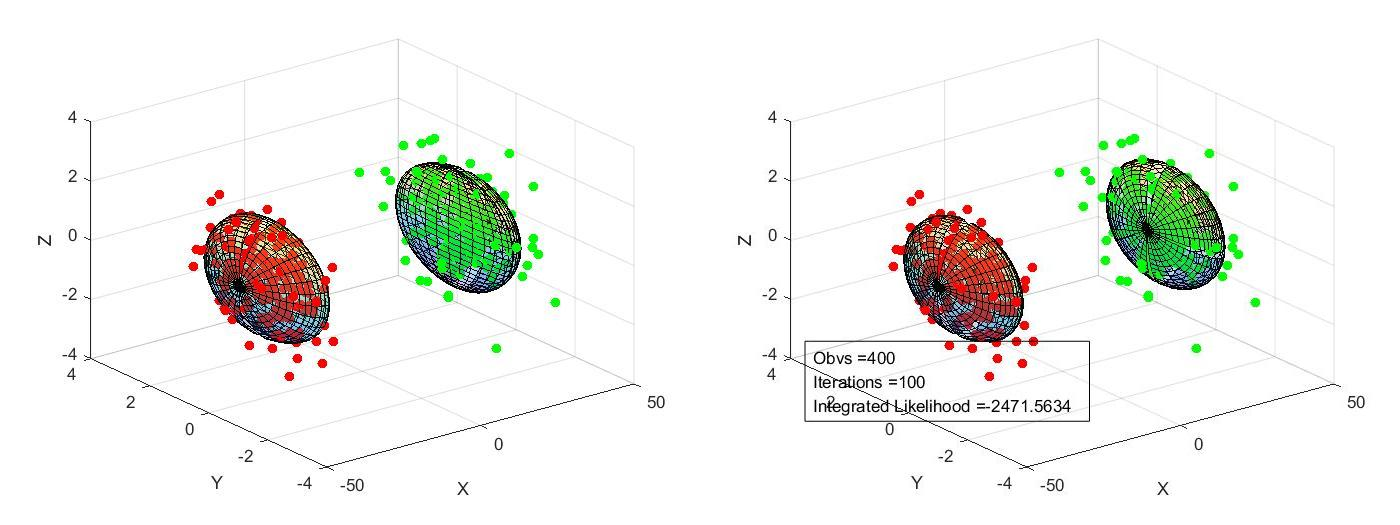
\includegraphics[width=0.75\textwidth]{syn.jpg}
\caption{Original synthetic data grouping and learning results}
\label{fig:syn1}
\end{figure}

\begin{figure}
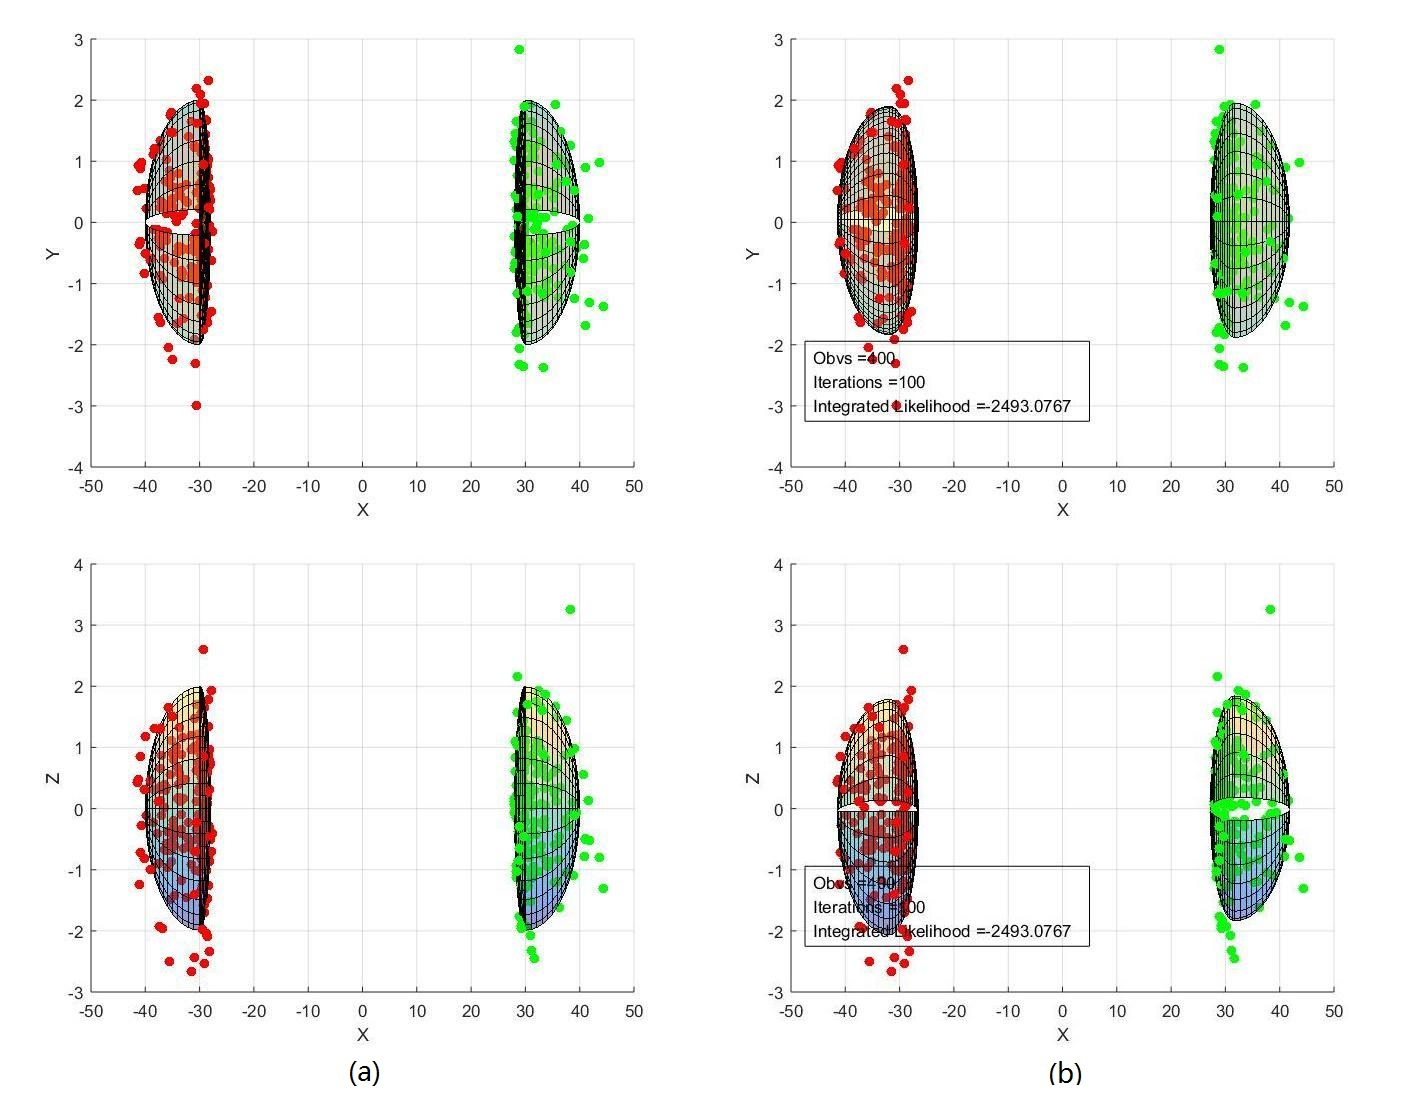
\includegraphics[width=0.75\textwidth]{xyzMerge.jpg}
\caption{(a) Original synthetic data grouping; (b) AGM clustering results}
\label{fig:syn2}
\end{figure}
The main goals of this section are feasibility analysis and efficiency evaluation of the AGM learning algorithm. The number of observations is set to 300 grouped into two clusters ($M$ = 2). Hyperparameters are set to $\gamma_j = 1$ \cite{Stephens2000} for sampling mixture weight $p_j$ from Eq. \eqref{eq:8}. $\eta$ and $\tau$ are considered as $d$-dimensional zero vectors in prior distributions of mixture parameter $\xi$.

Different proposed component numbers ($M' = 1,\dots,5$) are tested during the AGM learning process and the statistics are summarized in Table \ref{tab1}. In order to select the best number of components, we consider marginal likelihood as described in \cite{Bouguila2009}. The probability density functions are plotted for both original and estimated AGM components and the polylines show the trace of accepted moves for each component.

In terms of the best fit result, the accuracy is evaluated by calculating the Euclidean distance between original and estimated mixture parameter sets $\xi$ and $\hat{\xi}$ (Table \ref{tab2}). In summary, the estimation of mean is accurate because the Euclidean distance between $\mu_j$ and $\hat{\mu}_j$ is small but the distance between standard deviation $\sigma_{lj}, \sigma_{rj}$ and $\hat{\sigma}_{lj}, \hat{\sigma}_{rj}$ is slightly significant. However, this difference has not affected the clustering result.

 
\begin{table}
\caption{AGM Learning Statistics}

\begin{tabular}{|c|c|c|c|}
\hline
\multicolumn{1}{|p{2cm}|}{\centering \textbf{Component number $M'$}} & \multicolumn{1}{|p{2cm}|}{\centering \textbf{\textit{Moves accepted}}} & \multicolumn{1}{|p{2cm}|}{\centering \textbf{\textit{Acceptance ratio}}} & \multicolumn{1}{|p{2cm}|}{\centering \textbf{\textit{Marginal likelihood}}}\\
\hline
1 & 22 & 7.33\% & -1596.143  \\
2 & 11 & 3.67\% & -1500.370 \\
3 & 14 & 4.67\% & -1684.518 \\
4 & 63 & 21.00\% & -1522.148 \\
5 & 39 & 13.00\% & -1517.533 \\
\hline
\end{tabular}
\label{tab1}
\end{table}


\begin{table}
\caption{Accuracy Analysis ($M' = M = 2$)}

\begin{tabular}{|c|c|c|c|}
\hline
\multicolumn{1}{|p{2.5cm}|}{\centering \textbf{Component number $j = 1$}} & \multicolumn{1}{|p{2cm}|}{\centering \textbf{Mean \\($\mu_j$)}} & \multicolumn{1}{|p{2.5cm}|}{\centering \textbf{Left standard deviation ($\sigma_{lj}$)}} & \multicolumn{1}{|p{2.5cm}|}{\centering \textbf{Right standard deviation ($\sigma_{rj}$)}}\\
\hline
$\xi$ & [-15.00, 0.00] & [10.00, 1.00] & [1.00, 1.00]  \\
$\hat{\xi}$ & [-14.99, 0.25] & [4.77, 1.13] & [2.31, 1.88] \\
Euclidean Distance & 0.246 & 5.236 & 1.581 \\
\hline
\multicolumn{1}{|p{2.5cm}|}{\centering \textbf{Component number $j = 2$}} & \multicolumn{1}{|p{2cm}|}{\centering \textbf{Mean \\($\mu_j$)}} & \multicolumn{1}{|p{2.5cm}|}{\centering \textbf{Left standard deviation ($\sigma_{lj}$)}} & \multicolumn{1}{|p{2.5cm}|}{\centering \textbf{Right standard deviation ($\sigma_{rj}$)}}\\
\hline
$\xi$ & [15.00, 0.00] & [1.00, 1.00] & [10.00, 1.00]  \\
$\hat{\xi}$ & [14.02, -0.24] & [2.04, 1.04] & [5.70, 1.59] \\
Euclidean Distance & 1.010 & 1.036 & 4.338 \\
\hline
\end{tabular}
\label{tab2}
\end{table}

\subsubsection{Intrusion Detection}
\label{sec:2.5.2}

Along with the rapid growth of information technologies, personal and commercial behaviors tend to rely on computer network and Internet environments. However, based on the characteristics of networking, exposing sensitive privacy and valuable business secret online is extremely dangerous because accessibility and anonymity make network intrusions hard to be detected and traced, therefore, compromise network security. Cisco 2017 Annual Cybersecurity Report (ACR) \cite{Cisco2017} pointed out a crucial fact that more than one-third of organizations that experienced a breach in 2016 reported more than 20 percent of customer, opportunity and revenue loss. As a consequence, more than 90 percent of these organizations are improving threat defense technologies and processes by enhancing IT and security functions, increasing security training of employees and implementing risk mitigation techniques. Recently, machine learning-based intrusion detection solutions \cite{Buczak2016,Ashfaq2017} are drawing more attention because of their efficiency and flexibility. 

Earlier intrusion prevention approaches, such as authentication, avoiding programming errors and encryption, were proven as insufficient because along with the increasing of the complexity of network-based software systems, exploitable weaknesses are inevitable due to programming issues. Moreover, authentication and encryption are not always reliable since credentials could be leaked and encryption algorithm could also be compromised by applying powerful hacking techniques to make the attack feasible. In consequence, once intrusion happens, detection will be harder than prevention and sometimes victims could not be even aware of it. Therefore, many supervised data mining solutions were proposed in terms of misuse and anomaly detection systems by establishing known intrusion scenarios, normal usage patterns and the sequential interrelations between user operations to identify intrusion behaviors \cite{Lee1998}. However, the disadvantages of supervised intrusion detection systems are significant since predefined patterns and interrelations are inconsistent concerning the system upgrades and newly-founded intrusions which could lead to incessant intrusion detection system adjustment and affect its performance. Furthermore, inductive bias and overfitting problems caused by poor training datasets will also affect the accuracy of the systems. Therefore, researchers are paying more attention to unsupervised solution \cite{Bouguila2011,Azam2015} for seeking flexibility and robustness.

Therefore, we select NSL-KDD \cite{Tavallaee2009}, an improved KDDCUP'99 intrusion-detection data-set, as the testing target since redundant records have been removed from original dataset to avoid potential learning bias. Before applying the testing models onto the dataset, the data pre-processing is needed since discrete enumerated values must be translated to numerical ones and be normalized properly to lead an accurate result. Therefore, we substitute enumerated values with their numbers of occurrences which could reflect the density distribution of discrete values. Having all numerical data in hand, we apply feature scaling method to normalize numerical values between 0 to 1 as follows:

\begin{align}
x' = \frac{x - min(x)}{max(x) - min(x)}
\label{eq:13}
\end{align}
where $x$ and $x'$ denote original and normalized values. In this way we could use unified proposal distribution for every dimension with the same value of hyperparameter $\Sigma$ during random walk MCMC sampling step (Table \ref{tab4}).

K-means clustering algorithm \cite{Hartigan1979} is chosen for the comparison of accuracy. Testing data records with total amount of 25192 (20\% of NSL-KDD dataset) are clustered into two groups with 11743 intrusions and 13449 normal behaviors indicating components number $M' = 2$. In order to better evaluate the pros and cons of models, results derived from Gaussian mixture model (GMM) will also be taken into consideration. The comparison based on confusion matrices resulted from K-means, GMM and AGM model (Table \ref{tab5}) reveals the fact that based on a less accurate initialization given by K-means (60.85\%), GMM performs almost the same way as K-means and the difference between these two models is trivial. In contrast, AGM model makes a significant improvement with much higher accuracy rate (80.47\%) and precision percentage (96.86\%), while much lower false positive rate (4.26\%) illustrating AGM model is capable of effectively detecting intrusions from background noises. Compared with K-means and GMM, AGM model has a higher false negative rate (28.58\%) which means it tends to strictly identify normal behaviors as intrusions which could be mitigated by reducing dimensions of dataset using feature selection methodologies.

%\begin{table}
%\caption{Original NSL-KDD data records}
%
%\begin{tabular}{|c|c|}
%\hline
%\multicolumn{1}{|p{.3cm}|}{\centering\textbf{No}} & \multicolumn{1}{|p{9cm}|}{\centering\textbf{\textit{Value}}}\\
%\hline
%1 & {\tiny 0,tcp,ftp\_data,SF,491,0,0,0,0,0,0,0,0,0,0,0,0,0,0,0,0,0,2,2,0.00,0.00,0.00,0.00,1.00,0.00,0.00,150,25,0.17,0.03,0.17,0.00,0.00,0.00,0.05,0.00,normal}\\
%2 & {\tiny 0,udp,other,SF,146,0,0,0,0,0,0,0,0,0,0,0,0,0,0,0,0,0,13,1,0.00,0.00,0.00,0.00,0.08,0.15,0.00,255,1,0.00,0.60,0.88,0.00,0.00,0.00,0.00,0.00,normal} \\
%3 & {\tiny 0,tcp,private,S0,0,0,0,0,0,0,0,0,0,0,0,0,0,0,0,0,0,0,123,6,1.00,1.00,0.00,0.00,0.05,0.07,0.00,255,26,0.10,0.05,0.00,0.00,1.00,1.00,0.00,0.00,neptune} \\
%4 & {\tiny 0,tcp,http,SF,232,8153,0,0,0,0,0,1,0,0,0,0,0,0,0,0,0,0,5,5,0.20,0.20,0.00,0.00,1.00,0.00,0.00,30,255,1.00,0.00,0.03,0.04,0.03,0.01,0.00,0.01,normal} \\
%5 & {\tiny 0,tcp,http,SF,199,420,0,0,0,0,0,1,0,0,0,0,0,0,0,0,0,0,30,32,0.00,0.00,0.00,0.00,1.00,0.00,0.09,255,255,1.00,0.00,0.00,0.00,0.00,0.00,0.00,0.00,normal} \\
%6 & {\tiny 0,icmp,eco\_i,SF,18,0,0,0,0,0,0,0,0,0,0,0,0,0,0,0,0,0,1,1,0.00,0.00,0.00,0.00,1.00,0.00,0.00,1,16,1.00,0.00,1.00,1.00,0.00,0.00,0.00,0.00,ipsweep} \\
%\hline
%\end{tabular}
%\label{tab3}
%
%\end{table}

\begin{table}
\caption{Translation and Normalization of Internet Protocols (Enumerated Values)}

\begin{tabular}{|c|c|c|}
\hline
\multicolumn{1}{|p{2cm}|}{\centering \textbf{Internet Protocols}} & \multicolumn{1}{|p{2cm}|}{\centering \textbf{\textit{Number of Occurrences}}} & \multicolumn{1}{|p{2cm}|}{\centering \textbf{\textit{Normalized Values}}}\\
\hline
ICMP & 1655 & 0\\
UDP & 3011 & 0.071867 \\
TCP & 20526 & 1 \\
\hline
\end{tabular}
\label{tab4}

\end{table}

\begin{table}
\caption{Confusion Matrices and Statistics of K-means, GMM and AGM Models}

\begin{minipage}{.3\textwidth}


\textbf{K-means} \\
\begin{tabular}{|c|c|c|}
\hline
 & \multicolumn{1}{|p{1cm}|}{\centering \textbf{\textit{NF $^{\mathrm{a}}$}}} & \multicolumn{1}{|p{1cm}|}{\centering \textbf{\textit{F $^{\mathrm{b}}$}}}\\
\hline
\multicolumn{1}{|p{.3cm}|}{\centering \textbf{\textit{NF}}} & 2445 & 9298\\
\multicolumn{1}{|p{.3cm}|}{\centering \textbf{\textit{F}}} & 565 & 12884\\
\hline
\end{tabular}

\end{minipage}
\begin{minipage}{.3\textwidth}
    

\textbf{GMM} \\
\begin{tabular}{|c|c|c|}
\hline
 & \multicolumn{1}{|p{1cm}|}{\centering \textbf{\textit{NF}}} & \multicolumn{1}{|p{1cm}|}{\centering \textbf{\textit{F}}}\\
\hline
\multicolumn{1}{|p{.3cm}|}{\centering \textbf{\textit{NF}}} & 2464 & 9279\\
\multicolumn{1}{|p{.3cm}|}{\centering \textbf{\textit{F}}} & 584 & 12865\\
\hline

\end{tabular}

\end{minipage}
\begin{minipage}{.3\textwidth}
    

\textbf{AGM} \\
\begin{tabular}{|c|c|c|}
\hline
 & \multicolumn{1}{|p{1cm}|}{\centering \textbf{\textit{NF}}} & \multicolumn{1}{|p{1cm}|}{\centering \textbf{\textit{F}}}\\
\hline
\multicolumn{1}{|p{.3cm}|}{\centering \textbf{\textit{NF}}} & 11484 & 259\\
\multicolumn{1}{|p{.3cm}|}{\centering \textbf{\textit{F}}} & 5621 & 7828\\
\hline
\end{tabular}

\end{minipage}  

    

\begin{tabular}{|c|c|c|c|}
\hline
& \multicolumn{1}{|p{2cm}|}{\centering \textbf{\textit{K-means}}} & \multicolumn{1}{|p{2cm}|}{\centering \textbf{\textit{GMM}}} & \multicolumn{1}{|p{2cm}|}{\centering \textbf{\textit{AGM}}}\\
\hline
\multicolumn{1}{|p{3.2cm}|}{\centering \textbf{\textit{Accuracy}}} & 60.85\% & 60.85\% & 76.66\%\\
\multicolumn{1}{|p{3.2cm}|}{\centering \textbf{\textit{Precision}}} & 20.82\% & 20.98\% & 97.79\%\\
\multicolumn{1}{|p{3.2cm}|}{\centering \textbf{\textit{False Positive Rate}}} & 41.92\% & 41.90\% & 3.20\%\\
\multicolumn{1}{|p{3.2cm}|}{\centering \textbf{\textit{False Negative Rate}}} & 18.77\% & 19.16\% & 32.86\%\\
\hline
\multicolumn{3}{l}{$^{\mathrm{a}}$Non fault-prone, $^{\mathrm{b}}$Fault-prone.}
\end{tabular}

\label{tab5}
\end{table}


\subsubsection{Spam Filtering}
\label{sec:2.5.3}

\begin{table}[b]
\caption{AGM Statistics}

\begin{tabular}{|c|c|c|}
\hline
\multicolumn{1}{|p{2cm}|}{\centering \textbf{Init. Comp. Number $m$}} & \multicolumn{1}{|p{2cm}|}{\centering \textbf{\textit{Accuracy}}} & \multicolumn{1}{|p{2cm}|}{\centering \textbf{\textit{Integrated Likelihood}}}\\
\hline
$m=1$ & 55.64\% & $5.7074\mathrm{e}{5}$\\
$m=2$ & 51.21\% & $4.0543\mathrm{e}{5}$ \\
$m=3$ & 58.99\% & $8.4238\mathrm{e}{5}$ \\
\hline
\end{tabular}
\label{tab6}

\end{table}

Statistics reveal a crucial fact that more than 59\% of worldwide e-mail traffic is considered as unsolicited messages, also well known as spams, in 2017 \cite{Lab2018}. Most spams are irritating and resource-consuming, and some of them are extremely dangerous in terms of phishing scam, fee fraud, job offer scam, etc,. Since the damages of spam are persistent and significant not only for individuals but also for governments, companies and organizations, many spam filtering technologies have been proposed to address this issue and eliminate unwanted e-mails automatically over recent decades. 

Consequently, a well organized Spambase dataset \cite{Hopkins2018} is selected with attributes related to multiple spam textual features including spam word/character dictionaries and profiles of uninterrupted capital letter sequences. Data pre-processing includes Scaling-based data normalization which re-scales numerical values within the range between 0 and 1 and label extraction for generating confusion matrix. To better evaluate the performance and accuracy of AGM model under different initial number of components, the integrated likelihood \cite{Bouguila2009} values are given in Table \ref{tab6} to identify the best-fit result. Obviously, the result with initial component number $m=3$ has the largest integrated likelihood value ($8.4238\mathrm{e}{5}$). Therefore, we select it as the best-fit result and make horizontal comparison with GMM. Statistics in Table \ref{tab7} reveal the fact that comparing to GMM, AGM provides higher accuracy and precision, additionally, lower false positive rate and false negative rate indicate that AGM outperforms GMM. However, because of the nature of spambase, the performance of both mixture models is not satisfactory since most of spams cannot be identified. Therefore, data-based adjustment of the model might lead to a better result in the future. 

\begin{table}[h]
\caption{Confusion Matrices and Statistics of GMM and AGM}

\begin{tabular}{cc}
\begin{minipage}{.31\textwidth} 
\textbf{GMM} \\
\begin{tabular}{|c|c|c|}
\hline
 & \multicolumn{1}{|p{1cm}|}{\centering \textbf{\textit{NF $^{\mathrm{a}}$}}} & \multicolumn{1}{|p{1cm}|}{\centering \textbf{\textit{F $^{\mathrm{b}}$}}}\\
\hline
\multicolumn{1}{|p{.4cm}|}{\centering \textbf{\textit{NF}}} & 35 & 1778\\
\multicolumn{1}{|p{.4cm}|}{\centering \textbf{\textit{F}}} & 295 & 2493\\
\hline
\end{tabular}
\end{minipage}

\begin{minipage}{.31\textwidth}    
\textbf{AGM} \\
\begin{tabular}{|c|c|c|}
\hline
 & \multicolumn{1}{|p{1cm}|}{\centering \textbf{\textit{NF}}} & \multicolumn{1}{|p{1cm}|}{\centering \textbf{\textit{F}}}\\
\hline
\multicolumn{1}{|p{.4cm}|}{\centering \textbf{\textit{NF}}} & 249 & 1564\\
\multicolumn{1}{|p{.4cm}|}{\centering \textbf{\textit{F}}} & 323 & 2465\\
\hline
\end{tabular}
\end{minipage}  
\end{tabular}


\begin{tabular}{|c|c|c|}
\hline
 & \multicolumn{1}{|p{1.2cm}|}{\centering \textbf{\textit{GMM}}} & \multicolumn{1}{|p{1.2cm}|}{\centering \textbf{\textit{AGM}}}\\
\hline
\multicolumn{1}{|p{4cm}|}{\centering \textbf{\textit{Accuracy}}}  & 54.94\% & 58.99\%\\
\multicolumn{1}{|p{4cm}|}{\centering \textbf{\textit{Precision}}} & 1.93\% & 13.81\%\\
\multicolumn{1}{|p{4cm}|}{\centering \textbf{\textit{False Positive Rate}}}  & 41.63\% & 38.81\%\\
\multicolumn{1}{|p{4cm}|}{\centering \textbf{\textit{False Negative Rate}}} & 89.39\% & 56.46\%\\
\hline
\multicolumn{3}{l}{$^{\mathrm{a}}$Non fault-prone, $^{\mathrm{b}}$Fault-prone.}
\end{tabular}

\label{tab7}
\end{table}

\subsubsection{Conclusion}
\label{sec:2.5.4}

This chapter firstly illustrated a new intrusion detection approach by applying asymmetric Gaussian mixtures with a fully Bayesian learning process which is achieved by applying a hybrid sampling-based MH-within-Gibbs learning algorithm. According to the experiment results, the AGM model is proved as an effective approach for clustering.
In spite of the advantages of AGM we mentioned above, some improvements are still needed to promote the accuracy and flexibility and mitigate the drawbacks. Therefore, we shall extend the Bayesian learning process and introduce model selection and feature selection methodologies to improve the performance in the case of high-dimensional datasets.


%\begin{acknowledgements}
%If you'd like to thank anyone, place your comments here
%and remove the percent signs.
%\end{acknowledgements}

% BibTeX users please use one of
%\bibliographystyle{spbasic}      % basic style, author-year citations
\bibliographystyle{spmpsci}      % mathematics and physical sciences
%\bibliographystyle{spphys}       % APS-like style for physics
\bibliography{shuai}   % name your BibTeX data base

% Non-BibTeX users please use
%\begin{thebibliography}{}
%%
%% and use \bibitem to create references. Consult the Instructions
%% for authors for reference list style.
%%
%\bibitem{RefJ}
%% Format for Journal Reference
%Author, Article title, Journal, Volume, page numbers (year)
%% Format for books
%\bibitem{RefB}
%Author, Book title, page numbers. Publisher, place (year)
%% etc
%\end{thebibliography}

\end{document}
% end of file template.tex

